225. \begin{figure}[ht!]
\center{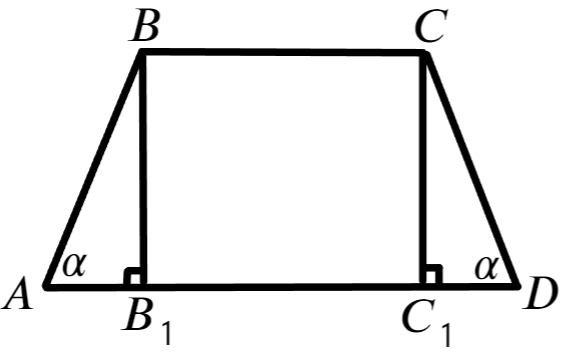
\includegraphics[scale=0.35]{g8-225.png}}
\end{figure}\\
Опустим высоты $BB_1$ и $CC_1.$ Тогда $\tg(\alpha)=\cfrac{BB_1}{AB_1}=\cfrac{CC_1}{C_1D}=\cfrac{h}{AB_1}=\cfrac{h}{C_1D},$ откуда $AB_1=C_1D=h\; ctg(\alpha).$ Поэтому $AD=AB_1+B_1C_1+C_1D=2h\; ctg(\alpha)+a.$ Найдём боковые стороны: $AB=CD=\cfrac{h}{\sin(\alpha)}.$ Таким образом, периметр трапеции равен $\cfrac{2h}{\sin(\alpha)}+a+2h\; ctg(\alpha)+a=2\left(\cfrac{h}{\sin(\alpha)}+h\; ctg(\alpha)+a\right),$ средняя линия трапеции равна $\cfrac{a+2h\; ctg(\alpha)+a}{2}=h\; ctg(\alpha)+a,$ а площадь равна $h(h\; ctg(\alpha)+a).$\\
